\chapter{Optimisation sans dérivées}
\label{chap:derivative-free}
\textit{(Brent, 1973)}

\section{Introduction}

Souvent, les dérivées sont indisponibles ou difficiles à calculer.
Exemples :
\begin{itemize}
    \item Le résultat d'une mesure expérimentale.
    \item Le résultat d'une simulation stochastique.
    \item $f$ est connue mais le calcul des dérivées est trop coûteux.
\end{itemize}

\section{Quelques solutions possibles}

\begin{itemize}
    \item \textbf{Différentiation automatique} : si un code binaire calcule $f$, on peut appliquer la différentiation automatique.
    
    \textit{Principe.} Si $f(x) = g(h(m(x)))$, on note $w = m(x)$, $y = h(w)$, $z = g(y)$.
    On utilise la règle de la chaîne (\textit{chain rule}) :
    \[
        f'(x) = \frac{\partial g}{\partial y} \bigg|_y \times \frac{\partial h}{\partial w} \bigg|_w \times \frac{\partial m}{\partial x} \bigg|_x.
    \]

    \item \textbf{Différences finies} : utiliser des différences finies pour approximer $\nabla f$ (et peut-être $\nabla^2 f$), puis appliquer les algorithmes des chapitres précédents.
    \textbf{Mais} cela peut être impossible à cause des approximations ou du bruit (\textit{noise}).
\end{itemize}

\section{Le problème du bruit}

Dans de nombreuses applications, la fonction objectif ressemble à :
\begin{equation}
    f(x) = h(x) + \phi(x),
\end{equation}
où $h$ est une fonction régulière (différentiable), et $\phi$ représente le bruit (possiblement indépendant de $x$).

L'approximation par différences finies du gradient $\nabla f(x)$ pour $\epsilon > 0$ est donnée par :
\[
    \nabla_\epsilon f(x) = \left( \frac{f(x+\epsilon e_i) - f(x-\epsilon e_i)}{2\epsilon} \right)_{i=1,\dots,n},
\]
où $e_i = (0, \dots, 1, \dots, 0)^\top$ est le $i$-ème vecteur de la base canonique.

\subsection{Niveau de bruit et erreur d'approximation}

Définissons le niveau de bruit local $\eta(x, \epsilon)$ par :
\begin{equation}
    \eta(x, \epsilon) = \sup_{\|z-x\|_\infty < \epsilon} |\phi(z)|.
\end{equation}

\begin{figure}[H]
\centering
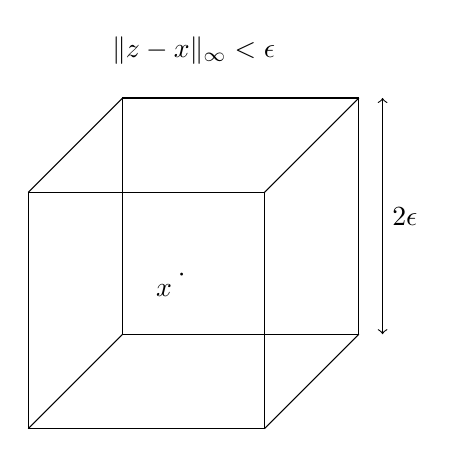
\begin{tikzpicture}[scale=1.5]
    % Cube 3D simple
    \draw (0,0) rectangle (2,2); % Face avant
    % x positioned more towards center of the 3D cube (accounting for perspective)
    \draw (1.3,1.3) node {$\cdot$} node[below left] {$x$};
    
    \draw (0,0) -- (0.8,0.8);
    \draw (2,0) -- (2.8,0.8);
    \draw (0,2) -- (0.8,2.8);
    \draw (2,2) -- (2.8,2.8);
    
    \draw (0.8,0.8) -- (2.8,0.8) -- (2.8,2.8) -- (0.8,2.8) -- cycle; % Face arrière
    
    % Dimensions
    \draw[<->] (3.0, 0.8) -- (3.0, 2.8) node[midway, right] {$2\epsilon$};
    
    \node at (1.4, 3.2) {$\|z - x\|_\infty < \epsilon$};
\end{tikzpicture}
\caption{Voisinage pris en compte pour le niveau de bruit.}
\label{fig:noise-cube}
\end{figure}

\begin{figureexplanation}
La figure~\ref{fig:noise-cube} représente le voisinage cubique $\|z - x\|_\infty < \epsilon$ autour du point $x$. Le niveau de bruit local $\eta(x, \epsilon)$ correspond à la plus grande amplitude du bruit $\phi(z)$ rencontrée à l'intérieur de ce cube de côté $2\epsilon$.
\end{figureexplanation}

On peut montrer que si $\nabla^2 h$ est $L$-Lipschitzienne dans le voisinage $\{z \mid \|z-x\|_\infty < \epsilon\}$, alors :
\begin{equation}
    \|\nabla_\epsilon f(x) - \nabla h(x)\|_\infty \le \underbrace{L \epsilon^2}_{\text{différences finies}} + \underbrace{\frac{\eta(x, \epsilon)}{\epsilon}}_{\text{bruit}}.
\end{equation}

On ne peut donc pas espérer une bonne approximation de $\nabla h(x)$ si le bruit est important, car réduire $\epsilon$ augmente l'amplification du bruit ($\eta/\epsilon$).

\begin{figure}[H]
\centering
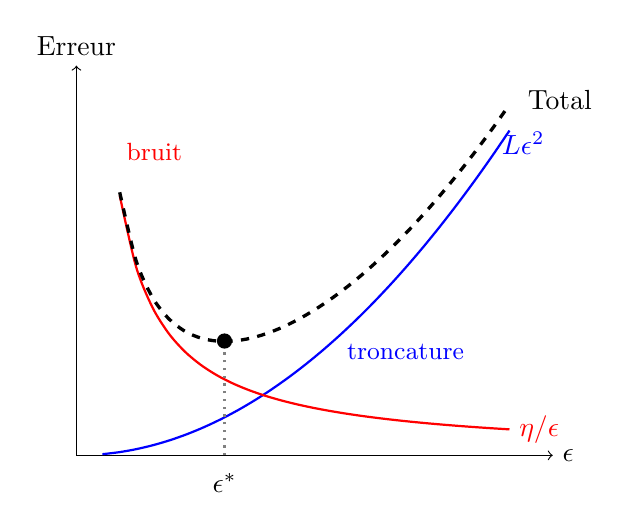
\begin{tikzpicture}[scale=1.1]
    % Axes
    \draw[->] (0,0) -- (5.5,0) node[right] {$\epsilon$};
    \draw[->] (0,0) -- (0,4.5) node[above] {Erreur};
    
    % Truncation error: L*epsilon^2 (quadratic, small near 0)
    \draw[domain=0.3:5, smooth, variable=\x, blue, thick] 
        plot ({\x}, {0.15*\x*\x});
    \node[blue, right] at (4.8, 3.6) {$L\epsilon^2$};
    \node[blue] at (3.8, 1.2) {\small troncature};
    
    % Noise amplification: eta/epsilon (hyperbolic, large near 0)
    \draw[domain=0.5:5, smooth, variable=\x, red, thick] 
        plot ({\x}, {1.5/\x});
    \node[red, right] at (5, 0.3) {$\eta/\epsilon$};
    \node[red] at (0.9, 3.5) {\small bruit};
    
    % Total error (sum)
    \draw[domain=0.5:5, smooth, variable=\x, black, very thick, dashed] 
        plot ({\x}, {0.15*\x*\x + 1.5/\x});
    \node[right] at (5.1, 4.1) {Total};
    
    % Optimal epsilon (minimum of total)
    % Derivative: 0.3*eps - 1.5/eps^2 = 0 => eps^3 = 5 => eps ~ 1.71
    \draw[dotted, gray, thick] (1.71, 0) -- (1.71, 1.32);
    \node[below] at (1.71, -0.1) {$\epsilon^*$};
    \fill (1.71, 1.32) circle (2.5pt);
\end{tikzpicture}
\caption{Compromis erreur de troncature vs amplification du bruit. L'erreur totale (pointillés) a un minimum en $\epsilon^*$.}
\label{fig:error-epsilon}
\end{figure}

\subsection{Exemple : Bruit stochastique}

Soient $X_1, \dots, X_n$ des variables aléatoires i.i.d. (indépendantes et identiquement distribuées) avec une moyenne $h(x)$ et une variance finie $\sigma^2$.

Alors le théorème central limite donne :
\[
    \sqrt{n} \left( \frac{1}{n} \sum_{i=1}^n X_i - h(x) \right) \xrightarrow{d} \mathcal{N}(0, \sigma^2).
\]
Approximativement (« Roughly ») :
\[
    \frac{1}{n} \sum_{i=1}^n X_i - h(x) \approx \frac{\sigma}{\sqrt{n}} G,
\]
où $G \sim \mathcal{N}(0, 1)$.
Cela montre que l'erreur décroît seulement en $1/\sqrt{n}$, ce qui peut nécessiter un très grand nombre d'échantillons pour réduire le bruit à un niveau acceptable pour les différences finies.

De sorte que :
\[
    \underbrace{\frac{1}{n} \sum_{i=1}^n X_i}_{\text{observé}}
    \simeq
    \underbrace{h(x)}_{\text{partie utile}}
    +
    \underbrace{\frac{\sigma}{\sqrt{n}} G}_{\text{bruit } \phi}.
\]
Dans cette situation, $\phi$ est indépendant de $x$, et $\phi$ est même non borné (car la loi normale n'est pas bornée).

\begin{quote}
    \textbf{Attention :} À partir de maintenant, nous supposons que $f$ a des dérivées continues, même si ces dernières ne seront pas utilisées dans les algorithmes.
\end{quote}

Nous proposons une sélection non exhaustive de méthodes.

\section{Méthodes basées sur un modèle (Model-based methods)}

\subsection{Idée générale}
L'idée est de construire un modèle $m_k$ (souvent quadratique) qui interpole la fonction $f$ sur un ensemble de points bien choisis.

Supposons qu'à l'étape $k$, nous disposons de l'ensemble de points interpolation $\mathcal{Y} = \{y_1, \dots, y_q\}$ avec $y_i \in \mathbb{R}^n$ pour $i=1, \dots, q$, et que l'itéré courant $x_k$ est l'un d'entre eux. De plus, aucun point dans $\mathcal{Y}$ n'a une valeur de fonction inférieure à celle de $f(x_k)$.

\subsection{Construction du modèle}

Notre modèle sera de la forme :
\begin{equation}
    m_k(x_k + p) = c + g^\top p + \frac{1}{2} p^\top G p,
\end{equation}
où $c \in \mathbb{R}$, $g \in \mathbb{R}^n$, et $G \in \mathbb{R}^{n \times n}$ est symétrique.

Nous déterminons $c$, $g$ et $G$ en imposant les conditions d'interpolation :
\begin{equation}
    m_k(y_i) = f(y_i), \quad i=1, \dots, q.
\end{equation}

Il y a $1 + n + \frac{n(n+1)}{2} = \frac{(n+1)(n+2)}{2}$ coefficients à ajuster.
Si nous choisissons $q = \frac{(n+1)(n+2)}{2}$, le système admet une solution unique (sous condition que les points soient bien positionnés).

Ensuite, nous calculons le pas $p$ en résolvant le sous-problème de confiance :
\begin{equation}
    \min_p m_k(x_k + p) \quad \text{sujet à } \|p\|_2 \le \Delta,
\end{equation}
pour un certain rayon de région de confiance $\Delta$.

\subsection{Mise à jour}
\begin{itemize}
    \item Si la décroissance est « importante », nous augmenterons $\Delta$ pour l'itération suivante.
    \item Sinon, nous mettons à jour l'ensemble $\mathcal{Y}$ ou nous réduisons le rayon de la région de confiance $\Delta$, et nous rejetons le pas.
\end{itemize}

\subsection{Initialisation et géométrie}
Pour l'algorithme complet (Algorithme 13), l'initialisation se fait souvent en prenant les $n+1$ sommets et les $\frac{n(n+1)}{2}$ milieux des arêtes d'un simplexe dans $\mathbb{R}^n$.

\begin{definition}[Simplexe]
    Un simplexe dans $\mathbb{R}^n$ est un ensemble de $n+1$ vecteurs $y_1, \dots, y_{n+1}$ dans $\mathbb{R}^n$.
    
    Le simplexe $\{y_1, \dots, y_{n+1}\}$ est dit \textbf{non dégénéré} si la matrice
    \[
        \begin{bmatrix}
            y_2 - y_1 & y_3 - y_1 & \cdots & y_{n+1} - y_1
        \end{bmatrix}
    \]
    est non singulière (c'est-à-dire que les directions sont indépendantes).
\end{definition}

\begin{figure}[H]
\centering
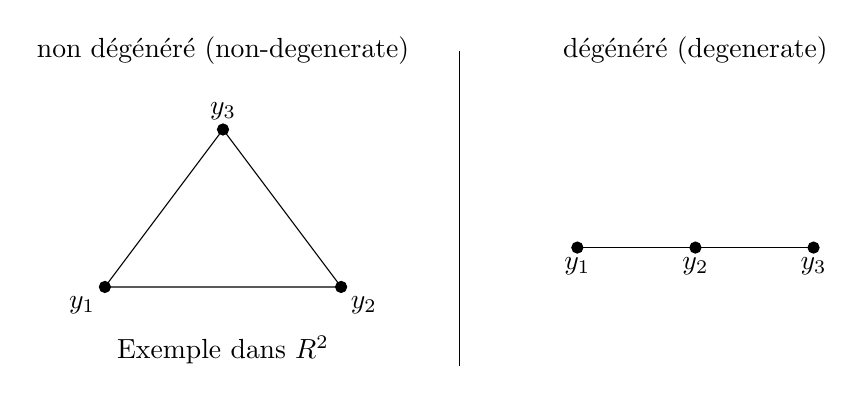
\begin{tikzpicture}[scale=1.0]
    % Non-degenerate simplex (Triangle) in R^2
    \begin{scope}[shift={(0,0)}]
        \node at (1.5, 3.0) {non dégénéré (non-degenerate)};
        \coordinate (A) at (0,0);
        \coordinate (B) at (3,0);
        \coordinate (C) at (1.5, 2);
        
        \draw (A) -- (B) -- (C) -- cycle;
        
        \filldraw (A) circle (2pt) node[below left] {$y_1$};
        \filldraw (B) circle (2pt) node[below right] {$y_2$};
        \filldraw (C) circle (2pt) node[above] {$y_3$};
        
        \node at (1.5, -0.8) {Exemple dans $\mathbb{R}^2$};
    \end{scope}
    
    % Vertical separator line
    \draw (4.5, -1) -- (4.5, 3);
    
    % Degenerate simplex (Aligned points)
    \begin{scope}[shift={(6,0)}]
        \node at (1.5, 3.0) {dégénéré (degenerate)};
        \coordinate (D) at (0, 0.5);
        \coordinate (E) at (1.5, 0.5);
        \coordinate (F) at (3, 0.5);
        
        \draw (D) -- (F); % Line connecting them
        
        \filldraw (D) circle (2pt) node[below] {$y_1$};
        \filldraw (E) circle (2pt) node[below] {$y_2$};
        \filldraw (F) circle (2pt) node[below] {$y_3$};
    \end{scope}
\end{tikzpicture}
\caption{Illustration d'un simplexe non dégénéré vs dégénéré dans $\mathbb{R}^2$.}
\label{fig:simplex-degenerate}
\end{figure}

\begin{figureexplanation}
La figure~\ref{fig:simplex-degenerate} illustre la notion de dégénérescence. À gauche, les vecteurs $y_2-y_1$ et $y_3-y_1$ sont linéairement indépendants, formant un vrai triangle (volume non nul). À droite, les points sont alignés : les vecteurs sont colinéaires, la matrice associée est singulière, et le simplexe est dégénéré (volume nul).
\end{figureexplanation}

\begin{algorithm}[H]
\caption{Méthode dérivée-free basée sur un modèle}
\label{alg:model-based-dfo}
Choose an interpolation set $Y = \{y^2, \ldots, y^q\}$ such that the linear system defined by $m_k(y^\ell) = f(y^\ell), \ell = 1, \ldots, q$ is nonsingular, and select $x_0$ as a point in this set such that $f(x_0) \le f(y^i)$ for all $y^i \in Y$. Choose an initial trust region radius $\Delta_0$, a constant $\eta \in (0,1)$, and set $k \leftarrow 0$\;
\Repeat{a convergence test is satisfied}{
    Form the quadratic model $m_k(x_k+)$ that satisfies the interpolation conditions $m_k(y^\ell) = f(y^\ell), \ell = 1, \ldots, q$\;
    Compute a step $p$ by approximately solving $\min_p m_k(x_k + p)$, subject to $\|p\|_2 \le \Delta$\;
    Define the trial point $x_k^+ = x_k + p$\;
    Compute the ratio $\rho = \dfrac{f(x_k) - f(x_k^+)}{m_k(x_k) - m_k(x_k^+)}$\;
    \If{$\rho \ge \eta$}{
        Replace an element of $Y$ by $x_k^+$\;
        Choose $\Delta_{k+1} \ge \Delta_k$\;
        Set $x_{k+1} \leftarrow x_k^+$\;
        Set $k \leftarrow k+1$ and go to the next iteration\;
    }
    \ElseIf{the set $Y$ need not be improved}{
        Choose $\Delta_{k+1} < \Delta_k$\;
        Set $x_{k+1} \leftarrow x_k$\;
        Set $k \leftarrow k+1$ and go to the next iteration\;
    }
    Invoke a geometry-improving procedure to update $Y$: at least one of the points in $Y$ is replaced by some other point, with the goal of improving the conditioning of $m_k(y^\ell) = f(y^\ell), \ell = 1, \ldots, q$\;
    Set $\Delta_{k+1} \leftarrow \Delta_k$\;
    Set $x_k^+ \leftarrow \hat{x}$ and recompute $\rho$ by $\rho = \dfrac{f(x_k) - f(x_k^+)}{m_k(x_k) - m_k(x_k^+)}$\;
    \If{$\rho \ge \eta$}{
        Set $x_{k+1} \leftarrow x_k^+$\;
    }
    \Else{
        Set $x_{k+1} \leftarrow x_k$\;
    }
    $k \leftarrow k + 1$\;
}
\end{algorithm}

\section{Méthodes de recherche par coordonnées ou par motifs (Coordinate or pattern-search methods)}

Partant de l'itéré courant, on regarde certains points le long de directions spécifiées, et on décide du pas.

\subsection{Recherche par coordonnées (Coordinate search)}
Aussi appelée \textit{coordinate descent}.

\paragraph{Idée.}
On cycle à travers les $n$ directions de coordonnées $e_1, \dots, e_n$.
On minimise $f$ le long de $e_i$, puis on recommence...

\paragraph{Attention.}
Cette méthode peut ne jamais approcher un point où le gradient s'annule (\textit{gradient-vanishing point}) !
Elle peut stagner aux coins de lignes de niveau anguleuses si les directions ne sont pas adaptées à la géométrie locale de la fonction.

Lorsque la convergence a lieu, elle peut être plus lente que la plus forte pente (\textit{steepest descent}).

\begin{figure}[H]
\centering
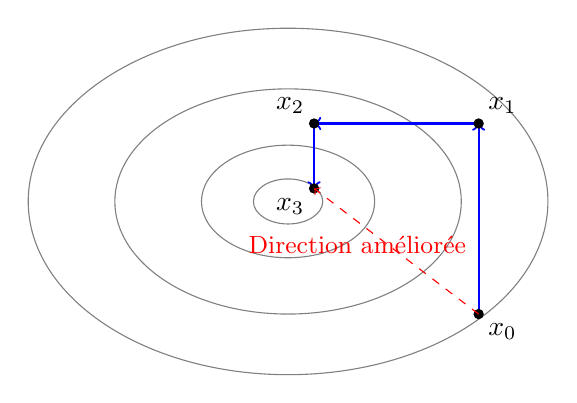
\begin{tikzpicture}[scale=1.1]
    % Contours (ellipses) - centered at origin
    \draw[gray] (0,0) ellipse (3cm and 2cm);
    \draw[gray] (0,0) ellipse (2cm and 1.3cm);
    \draw[gray] (0,0) ellipse (1cm and 0.65cm);
    \draw[gray] (0,0) ellipse (0.4cm and 0.26cm);

    % Starting point x0 on the outer ellipse
    % Ellipse: (x/3)^2 + (y/2)^2 = 1
    % At x=2.2: (2.2/3)^2 + (y/2)^2 = 1 => y = 2*sqrt(1-0.537) = 1.36
    % Let's place x0 at (2.2, -1.3) approximately on outer ellipse
    
    \coordinate (x0) at (2.2, -1.3);
    % Move vertically (along y) - coordinate search along e2
    \coordinate (x1) at (2.2, 0.9);
    % Move horizontally (along x) - coordinate search along e1
    \coordinate (x2) at (0.3, 0.9);
    % Move vertically again
    \coordinate (x3) at (0.3, 0.15);

    % Zigzag path with arrows
    \draw[->, thick, blue] (x0) -- (x1);
    \draw[->, thick, blue] (x1) -- (x2);
    \draw[->, thick, blue] (x2) -- (x3);

    % Point labels
    \node[below right] at (x0) {$x_0$};
    \node[above right] at (x1) {$x_1$};
    \node[above left] at (x2) {$x_2$};
    \node[below left] at (x3) {$x_3$};
    
    % Points markers
    \filldraw (x0) circle (1.5pt);
    \filldraw (x1) circle (1.5pt);
    \filldraw (x2) circle (1.5pt);
    \filldraw (x3) circle (1.5pt);

    % Improvement direction (direct path)
    \draw[dashed, red, ->] (x0) -- (x3);
    \node[red] at (0.8, -0.5) {\small Direction améliorée};
\end{tikzpicture}
\caption{Illustration de la recherche par coordonnées (zigzag) et de la lenteur potentielle.}
\label{fig:coordinate-zigzag}
\end{figure}

\begin{figureexplanation}
La figure~\ref{fig:coordinate-zigzag} montre que la méthode progresse en "escalier" (zig-zag). Les directions de coordonnées ne pointent pas nécessairement vers le minimum, forçant de nombreux petits pas.
\end{figureexplanation}

\paragraph{Amélioration possible.}
Effectuer $n$ itérations puis faire une recherche linéaire le long de la direction $(x_k - x_{k-n})$.

\subsection{Méthodes de recherche par motifs (Pattern-search methods)}

Cette classe de méthode généralise l'approche précédente.

\paragraph{Idée.}
Choisir un ensemble de directions de recherche $D_k$, et à chaque itération, évaluer $f$ à une longueur de pas donnée $\gamma_k$ le long de ces directions.
Si un point « plus intéressant » est trouvé, il devient le nouvel itéré.

\subsubsection{Algorithme 14 (Schéma général)}
On peut montrer qu'il existe des points d'accumulation stationnaires.
À l'étape $k$, soit $x_k$ l'itéré courant, $D_k$ l'ensemble courant de directions, et $\gamma_k$ la longueur de pas (\textit{step length}).

\begin{itemize}
    \item \textbf{Succès :} Si l'une des directions dans $D_k$ produit une décroissance significative, nous nous déplaçons vers ce nouveau point et nous augmentons le pas $\gamma_k$.
    \item \textbf{Échec :} Sinon, nous gardons $x_k$ et nous diminuons $\gamma_k$.
    \item Sous certaines conditions, l'ensemble $D_k$ peut être modifié.
\end{itemize}

\subsubsection{Conditions sur $D_k$}
Pour assurer la convergence, l'ensemble $D_k$ doit couvrir l'espace de manière suffisante.
Il doit y avoir au moins une direction de descente dans $D_k$, c'est-à-dire une direction $d \in D_k$ telle que :
\[
    \cos(\theta) = \frac{-\nabla f_k^\top d}{\|\nabla f_k\| \|d\|} > 0
\]

\paragraph{Condition de Zoutendijk (adaptée).}
Assurons-nous qu'il existe $\delta > 0$ tel que $\cos(\theta) > \delta$ pour au moins une direction.
On définit la mesure de qualité de l'ensemble de directions $\kappa(D_k)$ par :
\begin{equation}
    \kappa(D_k) = \min_{v \in \mathbb{R}^n} \max_{p \in D_k} \frac{v^\top p}{\|v\| \|p\|}
\end{equation}
La condition est alors : $\kappa(D_k) \ge \delta > 0$.

\textit{Interprétation :} Cette condition signifie que pour tout vecteur $v$, il existe une direction $p \in D_k$ qui forme un angle « suffisamment éloigné » de $\pi/2$ avec $v$. Plus précisément, le cosinus de l'angle entre $v$ et $p$ est borné inférieurement par une constante strictement positive $\delta$.

\subsubsection{Bornes sur le pas}
Il doit exister des constantes positives $\underline{\beta}, \bar{\beta}$ telles que pour tout $p \in D_k$ :
\[
    \underline{\beta} \le \|p\|_2 \le \bar{\beta}
\]
Le pas $\gamma_k$ doit capturer le diamètre effectif de la recherche.

Sous ces deux conditions, pour tout $k$, il existe un vecteur $p \in D_k$ tel que :
\begin{equation}
    -\nabla f_k^\top p \ge \kappa(D_k) \|\nabla f_k\| \|p\| \ge \delta \|\nabla f_k\| \underline{\beta}
\end{equation}
Cela garantit une décroissance suffisante tant que le gradient n'est pas nul.

\subsubsection{Ensembles $D_k$ possibles satisfaisant ces conditions}

Voici quelques exemples d'ensembles $D_k$ qui satisfont les conditions énoncées :

\paragraph{Exemple 1 : Directions canoniques et leurs opposées.}
\begin{equation}
    D_k = \{e_1, -e_1, e_2, -e_2, \dots, e_n, -e_n\}
\end{equation}
où $e_i$ est le $i$-ème vecteur de la base canonique.

\begin{figure}[H]
\centering
\begin{tikzpicture}[scale=1.2]
    % Axes for 2D case
    \draw[->, thick] (-2,0) -- (2,0) node[right] {$e_1$};
    \draw[->, thick] (0,-2) -- (0,2) node[above] {$e_2$};
    
    % Direction arrows
    \draw[->, blue, very thick] (0,0) -- (1.5,0) node[above right] {$e_1$};
    \draw[->, blue, very thick] (0,0) -- (-1.5,0) node[above left] {$-e_1$};
    \draw[->, red, very thick] (0,0) -- (0,1.5) node[above right] {$e_2$};
    \draw[->, red, very thick] (0,0) -- (0,-1.5) node[below right] {$-e_2$};
    
    \node at (0,-2.5) {Cas $n = 2$};
\end{tikzpicture}
\caption{Ensemble de directions $D_k = \{e_1, -e_1, e_2, -e_2\}$ dans $\mathbb{R}^2$.}
\label{fig:dk-canonical}
\end{figure}

\paragraph{Exemple 2 : Directions du simplexe.}
Pour $n \geq 1$, on définit :
\begin{align}
    n_i &= \frac{1}{2n} e - e_i, \quad i = 1, \dots, n, \\
    n_{n+1} &= \frac{1}{2n} e,
\end{align}
où $e = (1, \dots, 1)^\top \in \mathbb{R}^n$.

\begin{figure}[H]
\centering
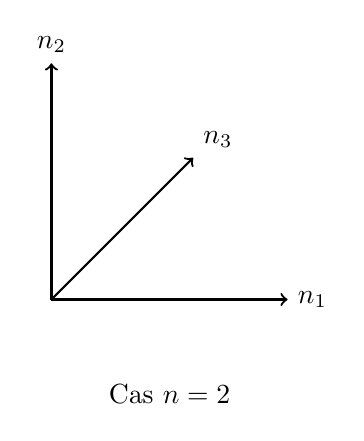
\begin{tikzpicture}[scale=1.5]
    % 3D coordinate system for illustration
    \draw[->, thick] (0,0) -- (2,0) node[right] {$n_1$};
    \draw[->, thick] (0,0) -- (0,2) node[above] {$n_2$};
    \draw[->, thick] (0,0) -- (1.2,1.2) node[above right] {$n_3$};
    
    \node at (1,-0.8) {Cas $n = 2$};
\end{tikzpicture}
\caption{Directions du simplexe dans $\mathbb{R}^2$.}
\label{fig:dk-simplex-directions}
\end{figure}

\begin{remarque}
\begin{itemize}
    \item On peut toujours enrichir l'ensemble $D_k$ avec des heuristiques intéressantes.
    \item Il n'est pas nécessaire d'examiner toutes les directions à chaque étape.
\end{itemize}
\end{remarque}

\begin{algorithm}[H]
\caption{Méthode de recherche par motifs}
\label{alg:pattern-search}
Given convergence tolerance $\gamma_{\text{tol}}$, contraction parameter $\theta_{\max}$, sufficient decrease function $\rho : [0,\infty) \to \mathbf{R}$ with $\rho$ an increasing function and $\frac{\rho(t)}{t} \to 0$ as $t \downarrow 0$\;
Choose initial point $x_0$, initial step length $\gamma_0 > \gamma_{\text{tol}}$, initial direction set $\mathcal{D}_0$\;
\For{$k = 1, 2, \ldots$}{
    \If{$\gamma_k \le \gamma_{\text{tol}}$}{
        \Stop\;
    }
    \If{$f(x_k + \gamma_k p_k) < f(x_k) - \rho(\gamma_k)$ for some $p_k \in \mathcal{D}_k$}{
        Set $x_{k+1} \leftarrow x_k + \gamma_k p_k$ for some such $p_k$\;
        Set $\gamma_{k+1} \leftarrow \phi_k \gamma_k$ for some $\phi_k \ge 1$ \Comment*[r]{increase step length}
    }
    \Else{
        Set $x_{k+1} \leftarrow x_k$\;
        Set $\gamma_{k+1} \leftarrow \theta_k \gamma_k$, where $0 < \theta_k \le \theta_{\max} < 1$\;
    }
}
\end{algorithm}

\section{Méthode du simplexe de Nelder-Mead}

\subsection{Principe général}

À chaque étape, nous gardons la trace de $n+1$ points dans $\mathbb{R}^n$, qui forment un simplexe.

À chaque itération :
\begin{itemize}
    \item On retire un point du simplexe.
    \item On le remplace par un point situé sur la droite qui joint l'ancien point au centroïde des $n$ meilleurs points.
    \item Le simplexe sera \textbf{étendu} (\textit{expanded}), \textbf{réfléchi} (\textit{reflected}), ou \textbf{contracté} (\textit{contracted}).
\end{itemize}

S'il n'existe pas de tel point qui améliore la fonction, on \textbf{rétrécit} (\textit{shrinks}) le simplexe vers le meilleur point.

\subsection{Notation et ordonnancement}

À une étape donnée, supposons que les sommets du simplexe sont ordonnés par valeur de fonction croissante :
\begin{equation}
    f(x_1) \leq f(x_2) \leq \cdots \leq f(x_{n+1})
\end{equation}
Ainsi, $x_1$ est le meilleur point (plus petite valeur de $f$), et $x_{n+1}$ est le pire point.

\subsection{Centroïde}

Le centroïde des $n$ meilleurs points (c'est-à-dire tous sauf $x_{n+1}$) est :
\begin{equation}
    \bar{x} = \frac{1}{n} \sum_{i=1}^{n} x_i
\end{equation}

\subsection{Points candidats}

Les points sur la droite joignant $x_{n+1}$ et $\bar{x}$ sont donnés par :
\begin{equation}
    \bar{x}(t) = \bar{x} + t(x_{n+1} - \bar{x}), \quad t \in \mathbb{R}
\end{equation}

\begin{figure}[H]
\centering
\begin{tikzpicture}[scale=1.3]
    % Simplex vertices
    \coordinate (x1) at (0, 0);
    \coordinate (x2) at (3, 0.3);
    \coordinate (x3) at (1.5, 2.5);
    
    % Centroid of x1 and x2
    \coordinate (xbar) at (1.5, 0.15);
    
    % Draw simplex
    \draw[thick] (x1) -- (x2) -- (x3) -- cycle;
    
    % Points
    \filldraw (x1) circle (2pt) node[below left] {$x_1$};
    \filldraw (x2) circle (2pt) node[below right] {$x_2$};
    \filldraw (x3) circle (2pt) node[above] {$x_3 = x_{n+1}$};
    \filldraw[blue] (xbar) circle (2pt) node[below] {$\bar{x}$};
    
    % Line from xbar through x3 and beyond
    % Extend the line: from t=-2 (below xbar) to t=1 (at x3)
    \draw[dashed, gray] ($(xbar)!-2!(x3)$) -- ($(xbar)!1.2!(x3)$);
    
    % Candidate points - TikZ (A)!t!(B) = A + t*(B-A)
    % which matches x̄(t) = x̄ + t*(x_{n+1} - x̄)
    \coordinate (xm2) at ($(xbar)!-2!(x3)$);     % t = -2 (expansion)
    \coordinate (xm1) at ($(xbar)!-1!(x3)$);     % t = -1 (reflection)
    \coordinate (xmhalf) at ($(xbar)!-0.5!(x3)$); % t = -1/2 (outside contraction)
    \coordinate (xphalf) at ($(xbar)!0.5!(x3)$);  % t = 1/2 (inside contraction)
    
    \filldraw[red] (xm2) circle (2pt) node[below] {$\bar{x}(-2)$};
    \filldraw[red] (xm1) circle (2pt) node[left] {$\bar{x}(-1)$};
    \filldraw[orange] (xmhalf) circle (2pt) node[left] {$\bar{x}(-\frac{1}{2})$};
    \filldraw[orange] (xphalf) circle (2pt) node[right] {$\bar{x}(\frac{1}{2})$};
    
    % Labels
    \node at (5, 1.5) {\small $t < 0$ : réflexion/expansion};
    \node at (5, 1) {\small $t > 0$ : contraction};
\end{tikzpicture}
\caption{Points candidats sur la droite joignant $x_{n+1}$ et le centroïde $\bar{x}$.}
\label{fig:nelder-mead-line}
\end{figure}

En pratique, on évalue :
\begin{itemize}
    \item $\bar{x}(-2)$ : expansion
    \item $\bar{x}(-1)$ : réflexion
    \item $\bar{x}(-\frac{1}{2})$ : contraction extérieure
    \item $\bar{x}(\frac{1}{2})$ : contraction intérieure
\end{itemize}

\begin{figure}[H]
\centering
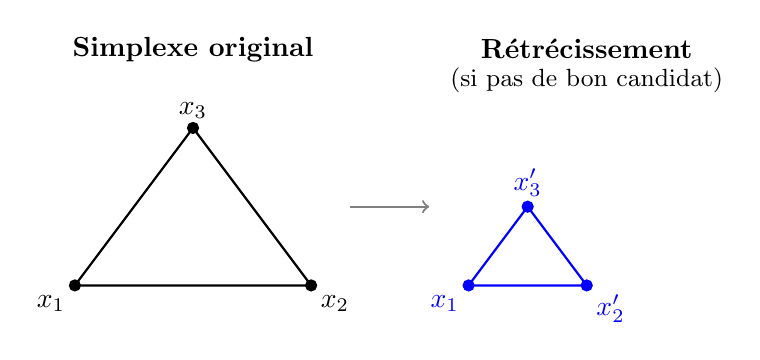
\begin{tikzpicture}[scale=1.0]
    % Original simplex
    \begin{scope}[shift={(0,0)}]
        \node at (1.5, 3) {\textbf{Simplexe original}};
        \coordinate (A) at (0,0);
        \coordinate (B) at (3,0);
        \coordinate (C) at (1.5, 2);
        
        \draw[thick] (A) -- (B) -- (C) -- cycle;
        \filldraw (A) circle (2pt) node[below left] {$x_1$};
        \filldraw (B) circle (2pt) node[below right] {$x_2$};
        \filldraw (C) circle (2pt) node[above] {$x_3$};
    \end{scope}
    
    % Arrow between the two simplexes (in global coordinates)
    \draw[->, thick, gray] (3.5, 1) -- (4.5, 1);
    
    % Shrink case (no good candidate)
    \begin{scope}[shift={(5,0)}]
        \node at (1.5, 3) {\textbf{Rétrécissement}};
        \node at (1.5, 2.6) {\small (si pas de bon candidat)};
        \coordinate (A2) at (0,0);
        \coordinate (B2) at (1.5, 0);
        \coordinate (C2) at (0.75, 1);
        
        \draw[thick, blue] (A2) -- (B2) -- (C2) -- cycle;
        \filldraw[blue] (A2) circle (2pt) node[below left] {$x_1$};
        \filldraw[blue] (B2) circle (2pt) node[below right] {$x_2'$};
        \filldraw[blue] (C2) circle (2pt) node[above] {$x_3'$};
    \end{scope}
\end{tikzpicture}
\caption{Opération de rétrécissement vers le meilleur point $x_1$.}
\label{fig:nelder-mead-shrink}
\end{figure}

\begin{figureexplanation}
La figure~\ref{fig:nelder-mead-shrink} illustre l'opération de rétrécissement (\textit{shrink}). Lorsqu'aucun des points candidats $\bar{x}(-2), \bar{x}(-1), \bar{x}(-\frac{1}{2}), \bar{x}(\frac{1}{2})$ n'améliore la fonction, le simplexe est rétréci vers le meilleur sommet $x_1$.
\end{figureexplanation}

\subsection{Remarques}

\begin{remarque}
L'ordre d'évaluation $\bar{x}(\frac{1}{2}), \bar{x}(-\frac{1}{2}), \bar{x}(-1), \bar{x}(-2)$ est assez standard dans les implémentations.
\end{remarque}

\begin{remarque}
À moins que l'étape de rétrécissement (\textit{shrinkage step}) ne soit effectuée, la quantité
\begin{equation}
    \frac{1}{n+1} \sum_{i=1}^{n+1} f(x_i)
\end{equation}
décroît à chaque étape.
\end{remarque}

\begin{remarque}
Pour la théorie de convergence, voir \cite{kelley1999detection} ou \cite{lagarias1995convergence}.
\end{remarque}

\subsection{Algorithme 15 : Méthode de Nelder-Mead}

\begin{algorithm}[H]
\caption{Une étape de la méthode de Nelder-Mead}
\label{alg:nelder-mead}
Compute the reflection point $\bar{x}(-1)$ and evaluate $f_{-1} = f(\bar{x}(-1))$\;
\If{$f(x_1) \le f_{-1} < f(x_n)$}{
    \Comment*[l]{Reflected point is neither best nor worst in the new simplex}
    Replace $x_{n+1}$ by $\bar{x}(-1)$ and go to the next iteration\;
}
\ElseIf{$f_{-1} < f(x_1)$}{
    \Comment*[l]{Reflected point is better than the current best, try to go further along this direction}
    Compute the expansion point $\bar{x}(-2)$ and evaluate $f_{-2} = f(\bar{x}(-2))$\;
    \If{$f_{-2} < f_{-1}$}{
        Replace $x_{n+1}$ by $x_{-2}$ and go to the next iteration\;
    }
    \Else{
        Replace $x_{n+1}$ by $x_{-1}$ and go to the next iteration\;
    }
}
\ElseIf{$f_{-1} \ge f(x_n)$}{
    \Comment*[l]{Reflected point is still worse than $x_n$, contract}
    \If{$f(x_n) \le f_{-1} < f(x_{n+1})$}{
        \Comment*[l]{try to perform ``outside'' contraction}
        Evaluate $f_{-1/2} = f(\bar{x}(-1/2))$\;
        \If{$f_{-1/2} \le f_{-1}$}{
            Replace $x_{n+1}$ by $x_{-1/2}$ and go to the next iteration\;
        }
    }
    \Else{
        \Comment*[l]{Try to perform ``inside'' contraction}
        Evaluate $f_{1/2} = f(\bar{x}_{1/2})$\;
        \If{$f_{1/2} < f_{n+1}$}{
            Replace $x_{n+1}$ by $x_{1/2}$ and go to the next iteration\;
        }
    }
    \Comment*[l]{Neither outside nor inside contraction was acceptable, shrink the simplex toward $x_1$}
    Replace $x_i \leftarrow \frac{1}{2}(x_1 + x_i)$ for $i = 2, 3, \ldots, n+1$\;
}
\end{algorithm}

\subsection{Illustration sur la fonction de Rosenbrock}

\begin{figure}[H]
\centering

\includegraphics[width=0.7\textwidth]{6.png}
\caption{Itérations de la méthode du simplexe de Nelder-Mead sur les courbes de niveau de la fonction de Rosenbrock.}
\label{fig:nelder-mead-rosenbrock}
\end{figure}

\begin{figureexplanation}
\textbf{Points clés à observer :}
\begin{itemize}
    \item \textbf{Méthode sans dérivée :} Nelder-Mead n'utilise aucune information sur le gradient, uniquement des évaluations de $f$. La trajectoire est donc moins directe que Newton ou BFGS.
    \item \textbf{Progression dans la vallée :} On peut observer comment le simplexe se déforme et s'adapte à la géométrie de la vallée de Rosenbrock par réflexions et contractions successives.
    \item \textbf{Robustesse vs efficacité :} La méthode converge malgré l'absence de dérivées, mais le nombre d'évaluations de $f$ est bien supérieur à la steepest descent (car toutes les autres méthodes utilisent aussi le gradient).
    \item \textbf{Cas d'usage :} Cette méthode est particulièrement utile lorsque les dérivées sont indisponibles ou trop coûteuses à calculer (simulations, mesures expérimentales).
\end{itemize}
\end{figureexplanation}
